%%%%%%%%%%%%%%%%%%%%%%%%%%%%%%%%%%%%%%%%%
% Large Colored Title Article
% LaTeX Template
% Version 1.1 (25/11/12)
%
% This template has been downloaded from:
% http://www.LaTeXTemplates.com
%
% Original author:
% Frits Wenneker (http://www.howtotex.com)
%
% License:
% CC BY-NC-SA 3.0 (http://creativecommons.org/licenses/by-nc-sa/3.0/)
%
%%%%%%%%%%%%%%%%%%%%%%%%%%%%%%%%%%%%%%%%%

%----------------------------------------------------------------------------------------
%	PACKAGES AND OTHER DOCUMENT CONFIGURATIONS
%----------------------------------------------------------------------------------------

\documentclass[letterpaper]{article}	 % A4 paper and 11pt font size
\usepackage[english]{babel} % English language/hyphenation
\usepackage[protrusion=true,expansion=true]{microtype} % Better typography
\usepackage{amsmath,amsfonts,amsthm} % Math packages
\usepackage[svgnames]{xcolor} % Enabling colors by their 'svgnames'
\usepackage{booktabs} % Horizontal rules in tables
\usepackage[margin=1.0in]{geometry}
\usepackage{hyperref}
\usepackage{xcolor}
\usepackage{float}
\usepackage{alltt}
\usepackage{graphicx}
\usepackage{lastpage} % Used to determine the number of pages in the document (for "Page X of Total")

%----------------------------------------------------------------------------------------
%	TITLE SECTION
%----------------------------------------------------------------------------------------

%----------------------------------------------------------------------------------------

\begin{document}

\begin{center}
    \Large
    \textbf{Assignment 1: \\ Matrix Multiplication}
    
    \vspace{0.4cm}
    \large
        
    \vspace{0.4cm}
    Lara Backer \\ Unmukt Gupta \\ Edward Tremel

\end{center}

%----------------------------------------------------------------------------------------
%  CONTENTS
%----------------------------------------------------------------------------------------

\section{Overview}

Matrix multiplication is one of the most fundamental computations required to solve linear systems, and as such is of vital importance in numerous computational applications. Therefore, reducing computation time for matrix multiplication calculations is an obvious method for increasing the efficiency of many solvers. \\

In this paper, we will be discussing the implementation and results from multiple methods for optimizing matrix multiplication of equation \ref{eq:mm}, with matrix dimensions M, N, and K. Results are compared to often-used matrix multiplication routines, such as those present in OpenBLAS, a basic blocked multiplication method, and a naive matrix multiplication routine. 

\begin{equation}
\text{C (M x N) = A (M x K) * B (K x N)}
\label{eq:mm}
\end{equation}

\section{Optimization Techniques}

\subsection{Blocking}
Blocking techniques take advantage of the temporal locality of inner loops. Each chunk, or 'block', of a matrix, is chosen so that the code loads the necessary block into cache for each loop, discarding the block when the loop is finished. Matrix multiplication is performed block by block. By knowing the cache level sizes, the block sizes can be chosen to fit within the cache and avoid cache misses, which will decrease code performance. \\ 

\noindent Each compute node on the totient cluster used to run this code has an Intel Xeon E5-2620 v3 processor. We first computed the cache sizes to try to figure out the optimal block sizes, as shown in the next subsections. We initially used the results from these calculations for block sizes, but as we will see later, further testing revealed that other block sizes performed even better. 


\subsubsection{Level 1 Cache}
The processor level 1 cache size is 32KB. To fit three blocks for A, B, and C for a square matrix and double matrix values (8 bytes), the formula to compute the optimal desired block size is:

\begin{equation}
\text{3*(block size)$^2$*(double size) = cache size}
\end{equation}

\noindent Thus, the maximum size for this blocking and for square matrices is 36x36.

\subsubsection{Level 2 cache}
For Xeon boards, the processor level 2 cache size is 256KB. In order to optimize for this cache as well, we performed two stages of blocking, one for the level 1 cache (smaller blocks), and one for level 2 (larger blocks). \\ \\

Using the same formula as for the level 1 cache, the maximum size for the level 2 blocking is 103. \\ \\

The first three lines of Figure \ref{fig:progression} show the improvement gained from adding one and two levels of blocking, respectively. We were surprised to see that the second level of blocking appeared to make little difference, but kept it for the small gains it produced at some sizes. 

\begin{figure}[H]
	\centering
	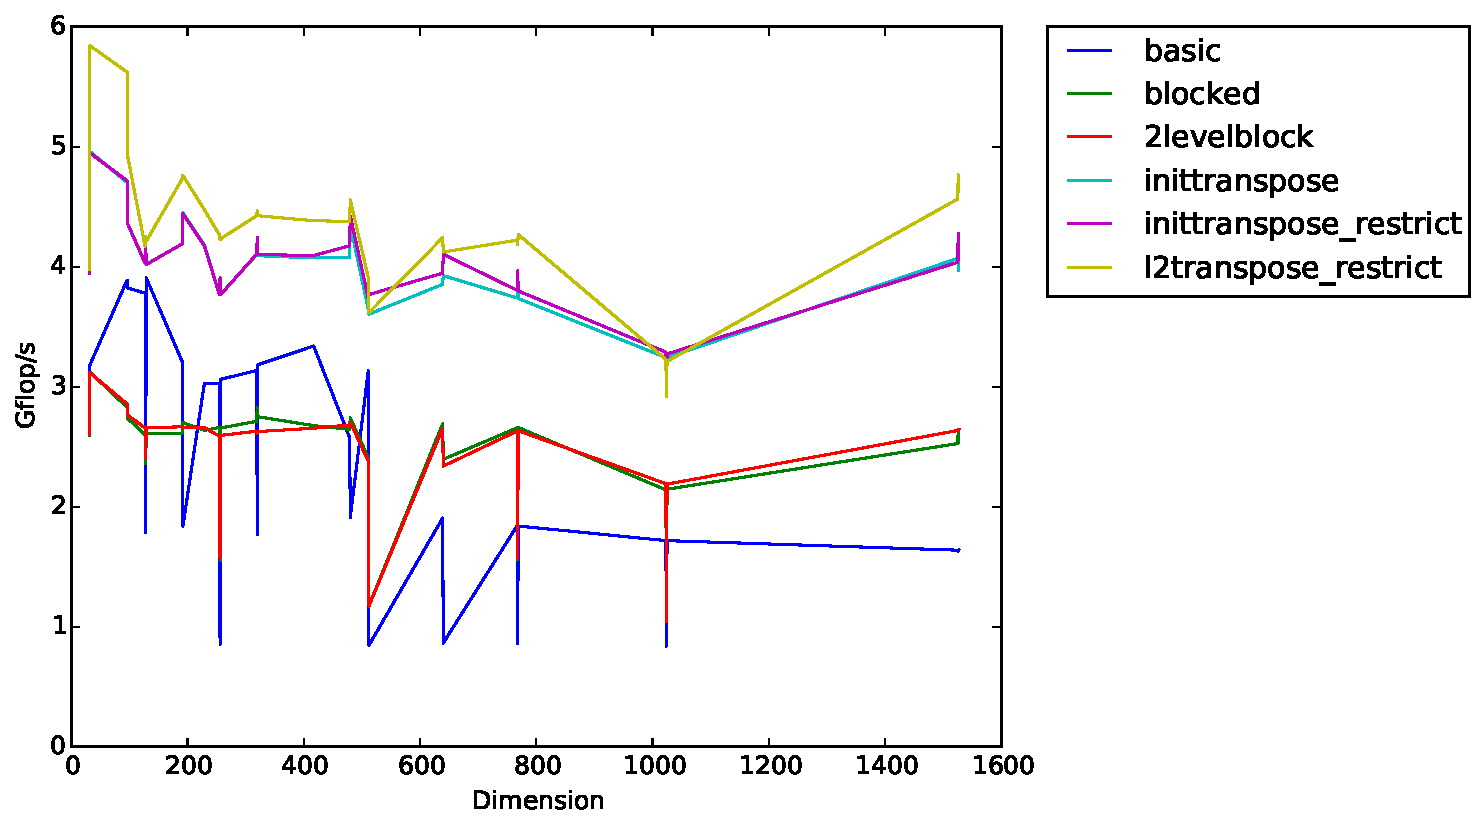
\includegraphics[width=.6\linewidth]{timing-progression.pdf}
	\caption{Performance of a series of optimization techniques. Blocking was performed with 36x36 small blocks and 103x103 large blocks}
	\label{fig:progression}
\end{figure}

\subsection{Copy Optimization}
Copy optimization improves spatial locality and reduces cache conflicts by copying fixed size blocks and storing them elsewhere for the computation. Due to the additional data storage, it primarily optimizes code for large matrix computations. We used copy optimization on matrix A, since we realized that the pattern of iteration over matrix A would be much more cache-efficient if it was stored in row-major rather than column-major order.

We first tried copying the entire input matrix A into a row-major format before iterating over it in blocks. The results of this optimization are the fourth line on Figure \ref{fig:progression}. As an alternative, to improve spatial locality for the block iterations, we tried copying each large block of matrix A to a row-major format before splitting it into small blocks. This did improve performance compared to transposing the entire input matrix at once, as shown on the last line of Figure \ref{fig:progression}.

\subsection{Compiler Hints}
C contains some special keywords that can be used to provide hints to the compiler about the layout of memory and allow it to use more aggressive optimizations. We tested the \texttt{restrict} keyword, which specifies that the memory region referenced by a pointer will not overlap with a memory region referenced by any other pointer in scope. This keyword could be applied to all pointers to matrices A, B, and C, since they are allocated in distinct sections of memory and the pointers are never used for any matrix other than their own.

The fifth line on Figure \ref{fig:progression} shows the results of adding the \texttt{restrict} keyword to all applicable pointers in our code that implemented the copy optimization with initial transposing. Unfortunately, this seemed to make little difference, but we kept it in future iterations of the code (such as the copy optimization at the large-block level).

\subsection{Index Order}
After implementing copy optimization, we tested all index orders for loops in the smallest blocked matrix multiplication routine (\texttt{dgemm\_basic}). We found that the default i,j,k ordering was already optimal for the code and blocking, as it was written.

\subsection{Block Size Tuning}
Although our calculations showed that block sizes of 36x36 and 103x103 should be optimal for the cache sizes of the cluster's Xeon boards, we experimented with a few other block sizes both smaller and larger than these, after implementing the copy optimization.

The results of different small- and large-block sizes for the implementation that copies matrix A at the large-block level are shown in Figure \ref{fig:l2blocking}. Surprisingly, it appears that the largest two block sizes, 64x64 for the small blocks and 256x256 for the large blocks, resulted in the best performance.

\begin{figure}[H]
\centering
  \centering
  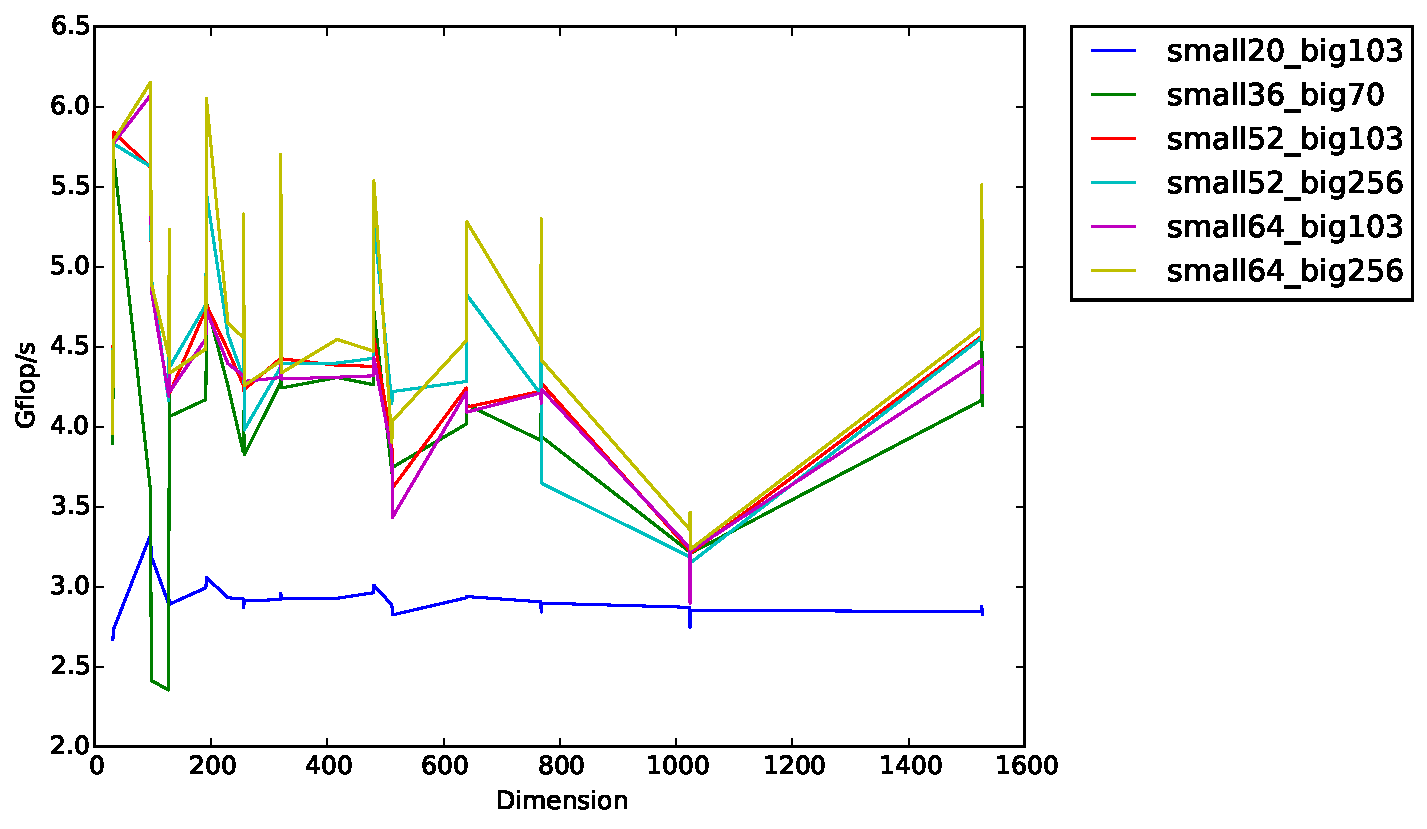
\includegraphics[width=.6\linewidth]{timing-blocksizes-l2transpose.pdf}
  \caption{Comparison of Different Blocking Sizes, with Copy Transpose at Large Blocks}
  \label{fig:l2blocking}
\end{figure}


\subsection{SSE Directives}

We hoped to be able to use SSE instructions to force matrix C to be written without being cached, since caching C does not improve performance and only takes up cache space that could be used by A and B. We tested a set of Intel intrinsic functions that are documented to use non-temporal storage instructions. We modified \texttt{dgemm\_basic} as follows:

\begin{verbatim}
void basic_dgemm(const int lda, const int M, const int N, const int K,
                 const double* restrict A, const double* restrict B, double* restrict C)
{
    int i, j, k;
        __m128d atemp,btemp,ctemp,cij
    for (i = 0; i < M; ++i) {
        for (j = 0; j < N; ++j) {
            cij = _mm_load_sd(&C[j*lda+i]);
                for(k = 0;k<K;++k) {
                        atemp = _mm_load_sd(&A[k*lda+i]);
                        btemp = _mm_load_sd(&B[j*lda+k]);
                        ctemp = _mm_mul_sd(atemp,btemp);
                        cij = _mm_add_sd(cij,ctemp);
            }
            _mm_stream_pd(&C[j*lda+i],cij);
        }
    }
}
\end{verbatim}

\begin{figure}[H]
  \centering
  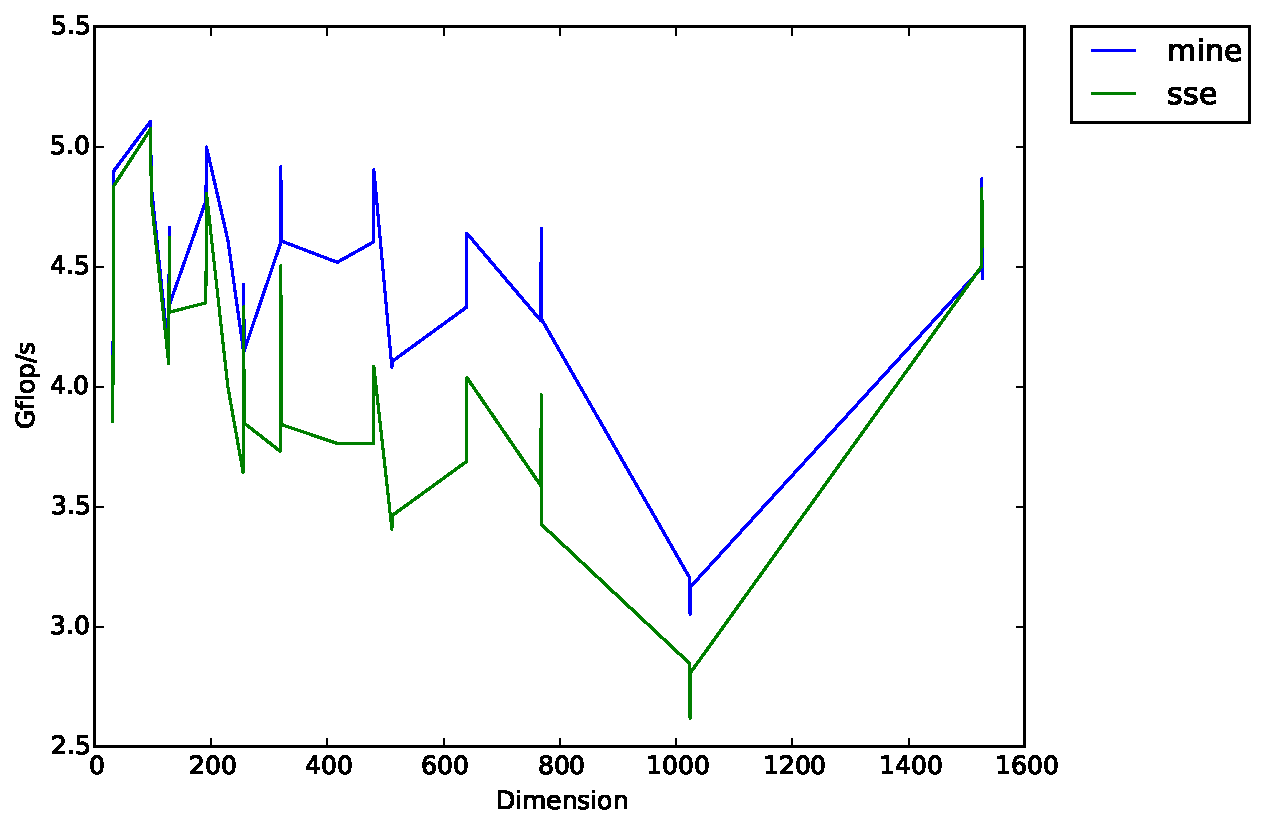
\includegraphics[width=.6\linewidth]{timing_sse.pdf}
  \caption{SSE Comparison Graph}
  \label{fig:sse}
\end{figure}
  
  As can be seen in Figure \ref{fig:sse}, the timings for the modified SSE code were actually worse when compared to the basic blocked dgemm\_mine code. 


\subsection{Compiler Flags}
Compiler flags that were found to improve performance were for this code are listed as follows: \\
\begin{itemize}
\item -O2: Maximizes speed, enables vectorization. Basic optimize flag. 
\item -mfpmath=sse: Enables XMM registers in floating point operations
\item -Ofast: Enables high level aggressive optimizations -O3, -no-prec-div, and -fp-model fast=2. 
\\ 

Additional options were tested, such as -ipo, -flto, and -march=native. However, none of the flags were actually shown to increase efficiency. A comparison of the timings for options with all bulleted flags (flags), just the -O3 flag (o3), and no flags used (noflags) is shown in Figure \ref{fig:flags}. 

\begin{figure}[H]
\centering
  \centering
  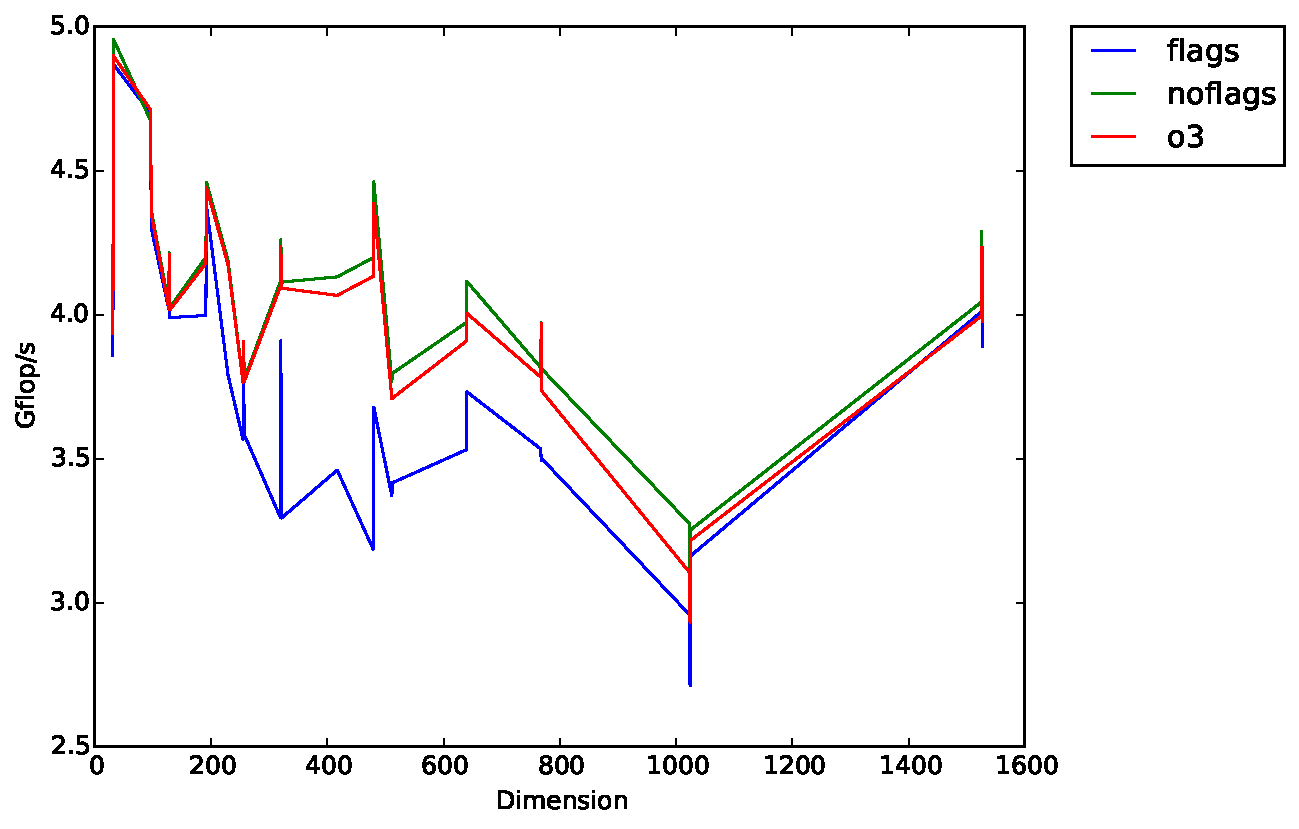
\includegraphics[width=.6\linewidth]{timing_flagcompare.pdf}
  \caption{Flag Comparison Graph}
  \label{fig:flags}
  \end{figure}

\end{itemize}

\section{Final Comparisons for Part 1}

After implementing all of the optimizations we found to improve performance, we were able to achieve a performance level a little less than halfway between the naive implementation of matrix multiply and the finely-tuned BLAS library. We also reduced the variation in speed with matrix dimension compared to the naive implementation, smoothing out many of the performance dips at powers of 2. 
The final timing graph for our code is shown in Figure \ref{fig:final}, compared to these two benchmarks.

\begin{figure}[H]
  \centering
  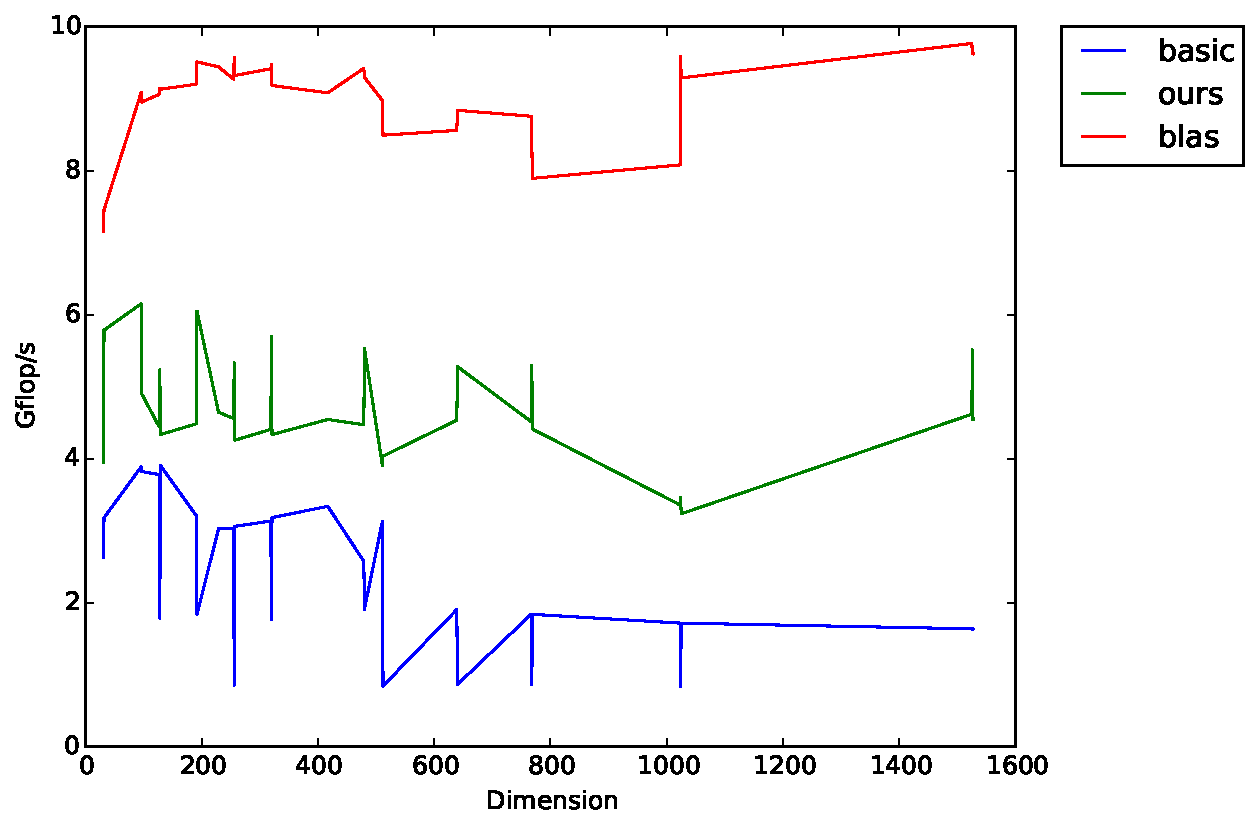
\includegraphics[width=.6\linewidth]{timing-final-comparison.pdf}
  \caption{Our optimized implementation compared to the naive matrix multiply and the BLAS library code.}
  \label{fig:final}
\end{figure}

\section{Revising for Part 2}

After receiving feedback from part 1 of this project, we decided to explore several new optimizations for part 2. One idea was to leave the matrices in column-major order and change the loop order to j-k-i to achieve the same cache-friendly access pattern without the overhead of coyping. Another was to test some additional compiler flags that we neglected to test initially, such as -funroll-loops. The idea that turned out to make the biggest difference, however, was rewriting the kernel of the inner loop to use AVX vector instructions to multiply small blocks of the matrices. This significantly changed our code and made many of the optimizations we found in Stage 1 obsolete, but it resulted in a large improvement.

\subsection{Index Order Revisited}
One of the groups that gave us feedback pointed out that transposing matrix A to row-major format was equivalent to a loop order that used the cache more efficiently, so we decided to see if we could eliminate the overhead of copying by using a different loop order. Other groups found that the j-k-i index order for loops had the best performance, so we compared our code from stage 1 to a non-copying version that used j-k-i index ordering. As Figure \ref{fig:copying-looporder} shows, we found that our transpose technique with standard loop ordering actually outperformed j-k-i loop ordering despite the overhead of copying.

\begin{figure}[H]
	\centering
	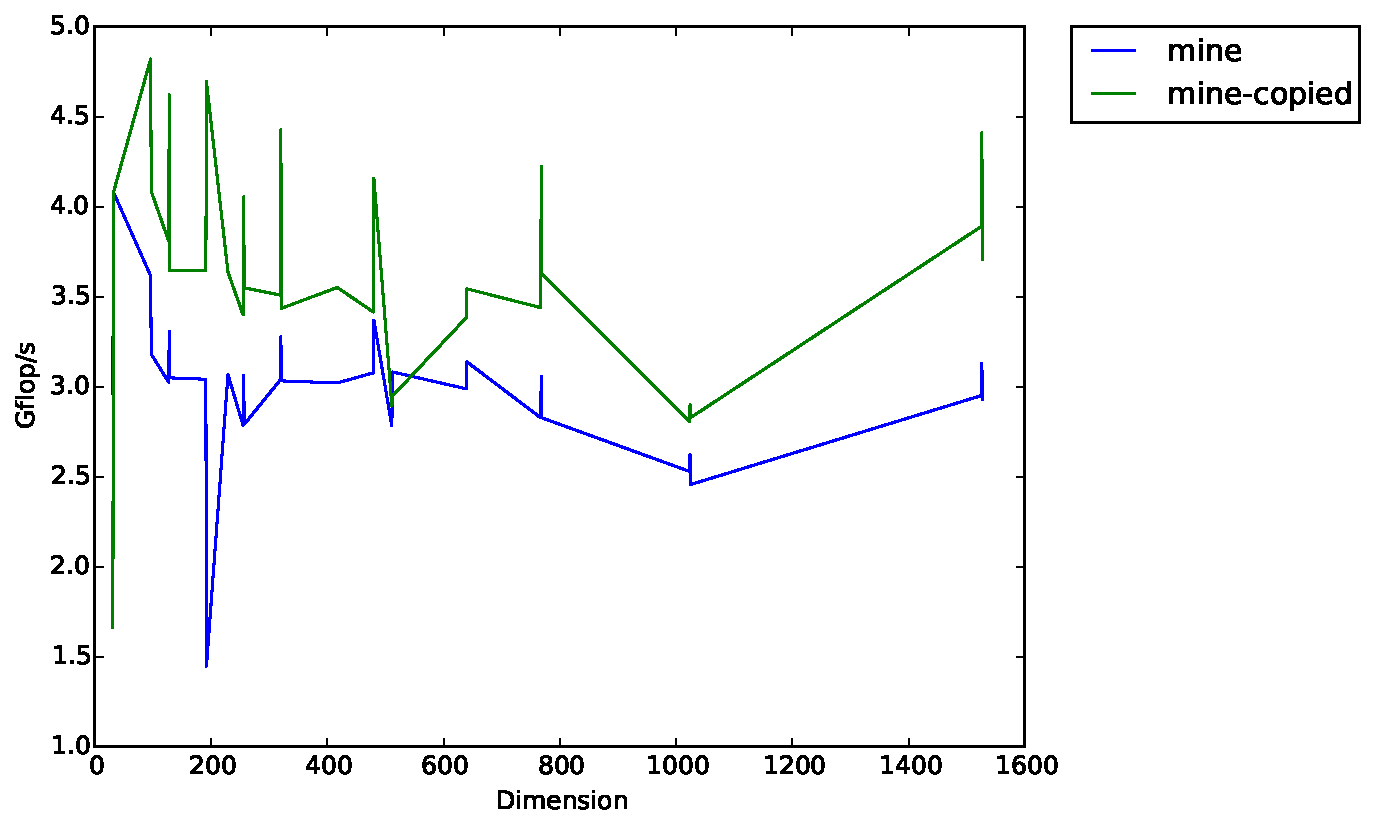
\includegraphics[width=.6\linewidth]{timing-copying_looporder.pdf}
	\caption{Loop reordering vs. copying and transposing}
	\label{fig:copying-looporder}
\end{figure}

\subsection{Compiler Flags Revisited}
We tested some additional optimizing compiler flags on our code from stage 1, including -funroll-loops and -aggressive. Results are shown in Figure \ref{fig:stage1-flags}. Although the flags still made only marginal difference, the -O3 and -aggressive flags seemed to help.

\begin{figure}[H]
	\centering
	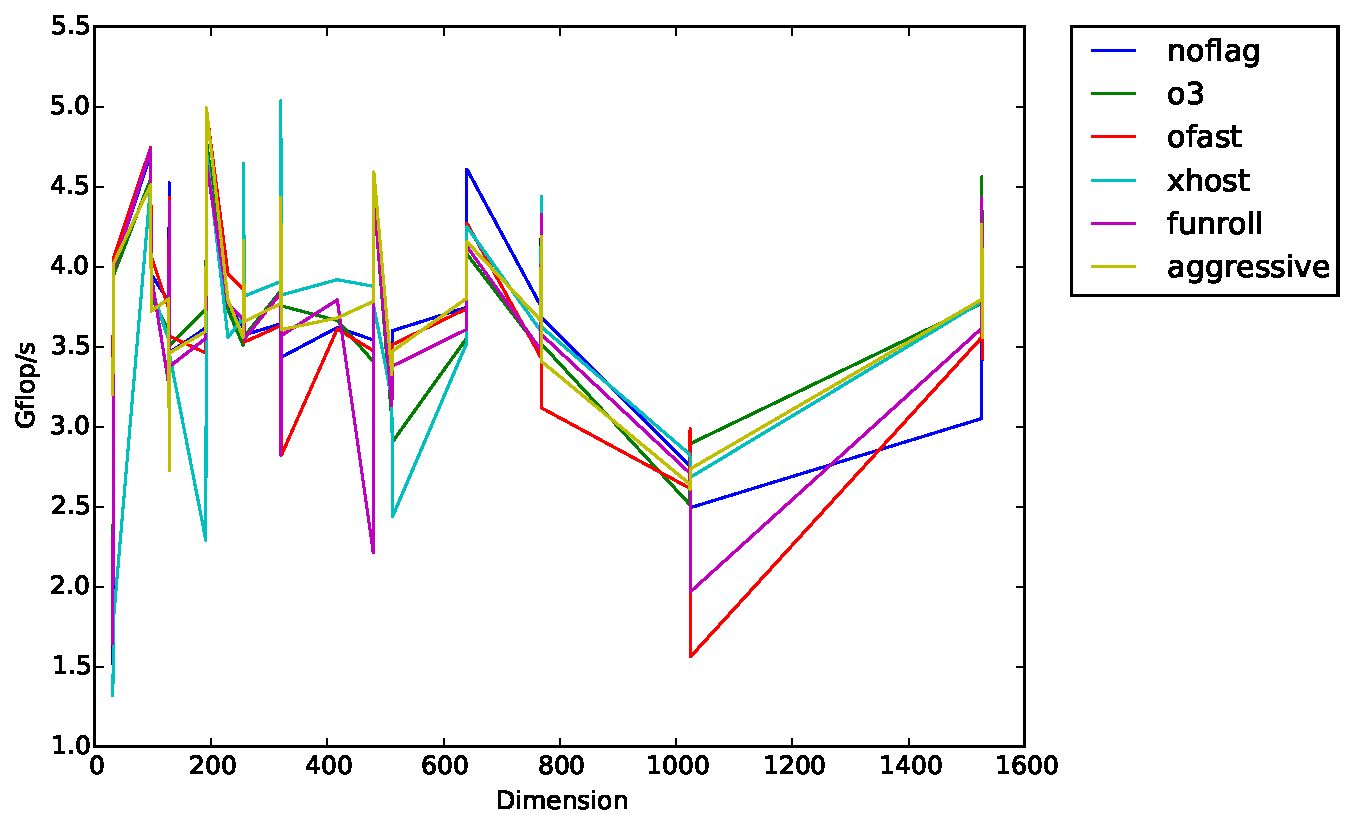
\includegraphics[width=.6\linewidth]{timing-flags_stage1.pdf}
	\caption{Additional compiler flags not tested in Stage 1}
	\label{fig:stage1-flags}
\end{figure}

\subsection{AVX Instructions}
We tried rewriting the ``kernel'' of our code, the inner loop that multiplies a small section of the matrices, to use Intel AVX vector instructions instead of naive C multiplication. This limited the way we could use the kernel because the AVX instructions require aligned memory and can only be used to multiply sets of 4 matrix elements at a time (the number of double-precision numbers that can fit in an AVX register). Our lowest-level routine became \texttt{dgemm\_4x4}, multiplying a fixed-size square of the two matrices, which means our small block size was effectively fixed at 4. Also, the input matrices had to be zero-padded so that their sizes were a multiple of 4.

\begin{figure}[H]
	\centering
	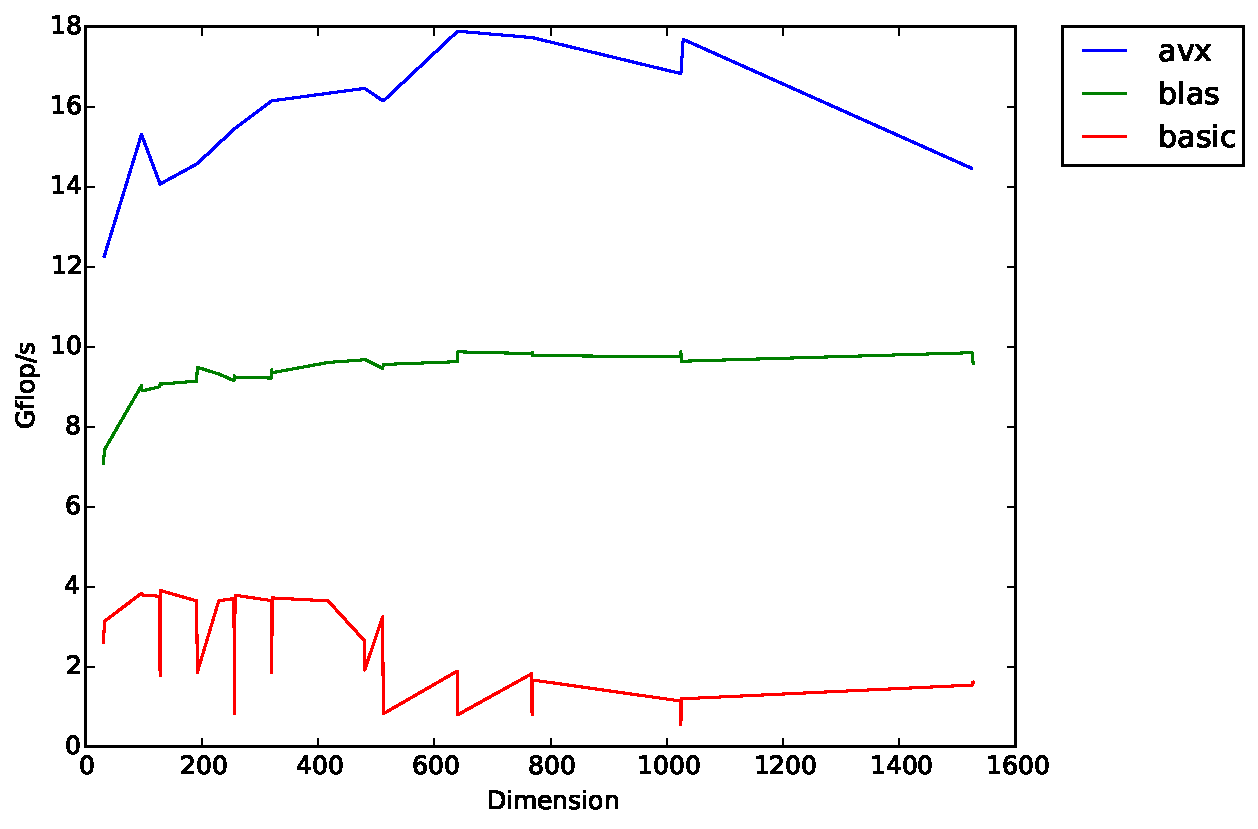
\includegraphics[width=.6\linewidth]{timing-avx_initial.pdf}
	\caption{Re-implementing the kernel using Intel AVX instructions}
	\label{fig:avx-initial}
\end{figure}

The code using AVX instructions is too long to include here, but it can be seen in the file \texttt{dgemm\_avx.c} included in our pull request. Our initial implementation using AVX instructions used a simple initial copy optimization (without transposing) to copy the matrices into new aligned memory and add zero-padding to the nearest multiple of 4, and did not implement multi-level blocking, using only the mandated 4x4 tiles to iterate the AVX kernel. The results can be seen in Figure \ref{fig:avx-initial} (compared to BLAS for reference). At over 14 GFlops/s, this is already a huge improvement over our best optimizations from Stage 1, despite the fact that we removed several of them.

\subsection{Improving the AVX Version}
After concluding that the AVX code was far superior to our Stage 1 code, we experimented with re-introducing some optimizations to this version.

\subsubsection{Compiler Hints}
Our initial implementation with AVX instructions did not use the \texttt{restrict} keyword on the pointers to matrices A, B, and C, but it did not use any pointers in an overlapping manner. We added the \texttt{restrict} keyword to every \texttt{double *} pointer, as we did for Stage 1. As shown in Figure \ref{fig:avx-restrict}, we found that it made some improvements at small matrix sizes, so we kept these keywords in further iterations of our code.. 

\begin{figure}[H]
	\centering
	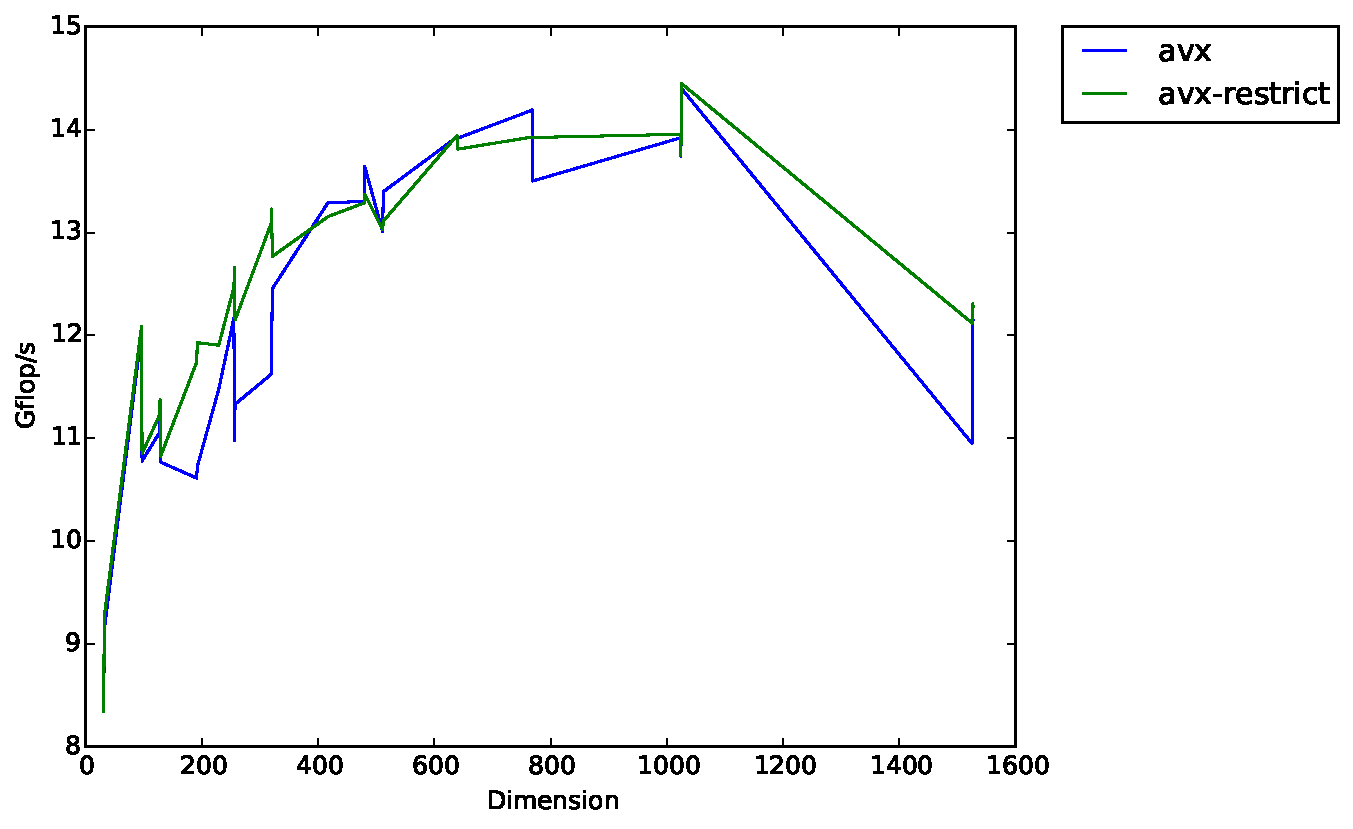
\includegraphics[width=.6\linewidth]{timing-restrict.pdf}
	\caption{Adding the \texttt{restrict} compiler hint}
	\label{fig:avx-restrict}
\end{figure}

\subsubsection{Blocking}
We initially tried implementing a two-level blocking scheme similar to the one we used in Stage 1, using three nested loops. However, this actually made the AVX code's performance worse. Then we found a publicly-available example from the University of Texas\footnote{\url{http://wiki.cs.utexas.edu/rvdg/HowToOptimizeGemm/Optimization\_4x4\_13/}} that showed an AVX kernel similar to ours with a simpler large blocking scheme. We implemented this blocking scheme using a large block size of 768, and it significantly improved performance at large matrix sizes without hurting performance at small sizes.


\subsubsection{Copy Optimization}
Due to the way matrix B is accessed in our AVX code it no longer made sense to copy only small blocks of matrix B at a time, but we could move the copying of matrix A to a lower level once we had implemented blocking. Since copying at a lower level was better than initial copying of the whole matrix for our Stage 1 code, we tried copying and padding matrix A in small slices 4 elements wide and a large block high, in the inner block-level loop. This provided marginal improvement, but we include it in the results shown in Figure \ref{fig:avx-blocked}.

\begin{figure}[H]
	\centering
	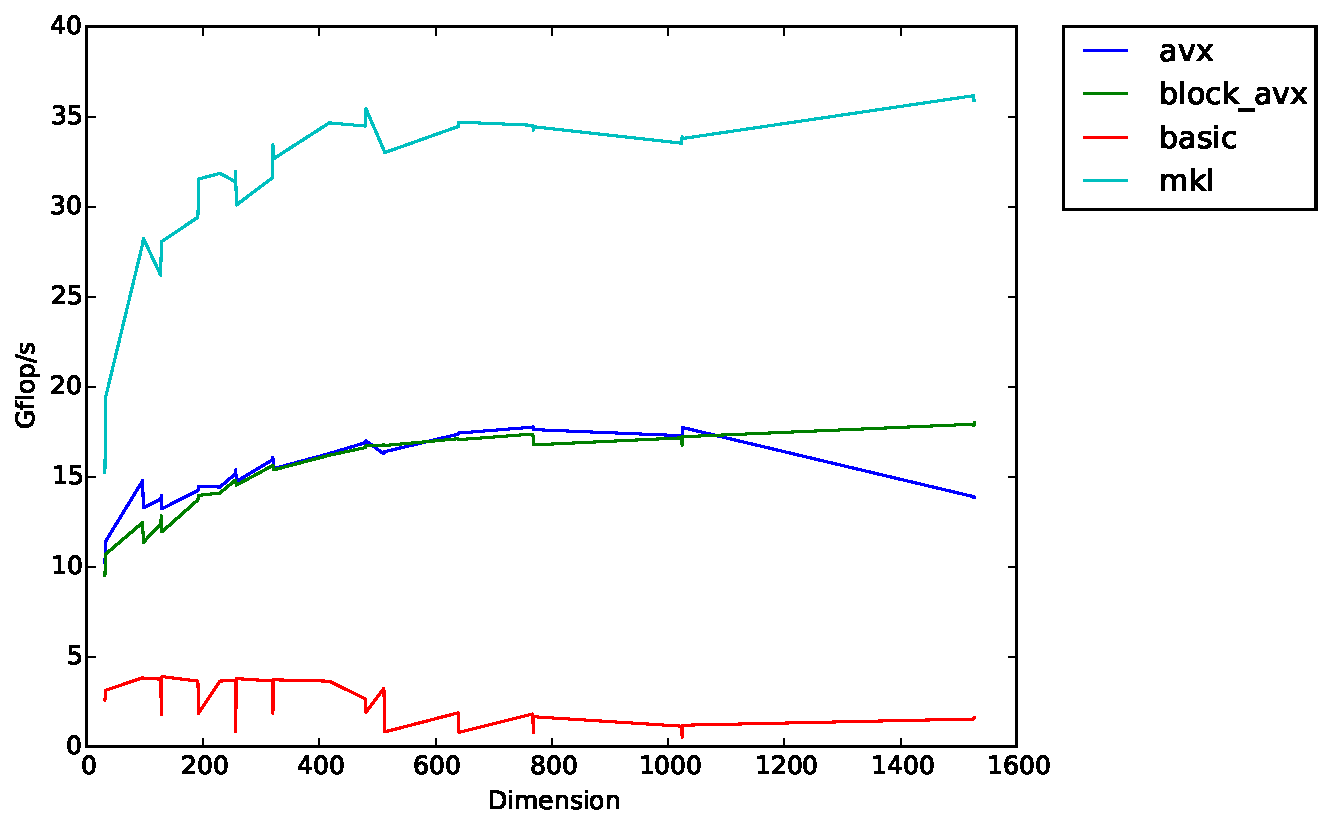
\includegraphics[width=.6\linewidth]{timing-avx_blocked.pdf}
	\caption{Adding large-level blocking to the AVX version of the code.}
	\label{fig:avx-blocked}
\end{figure}

\subsubsection{Compiler Flags, Again}
We experimented with the compiler flags again with both the non-blocked and blocked versions of the AVX code. Figure \ref{fig:avx-flags-noblocking} shows the results for the non-blocked version, and Figure \ref{fig:avx-flags-blocking} shows the results for the blocked version. 

\begin{figure}[H]
	\centering
	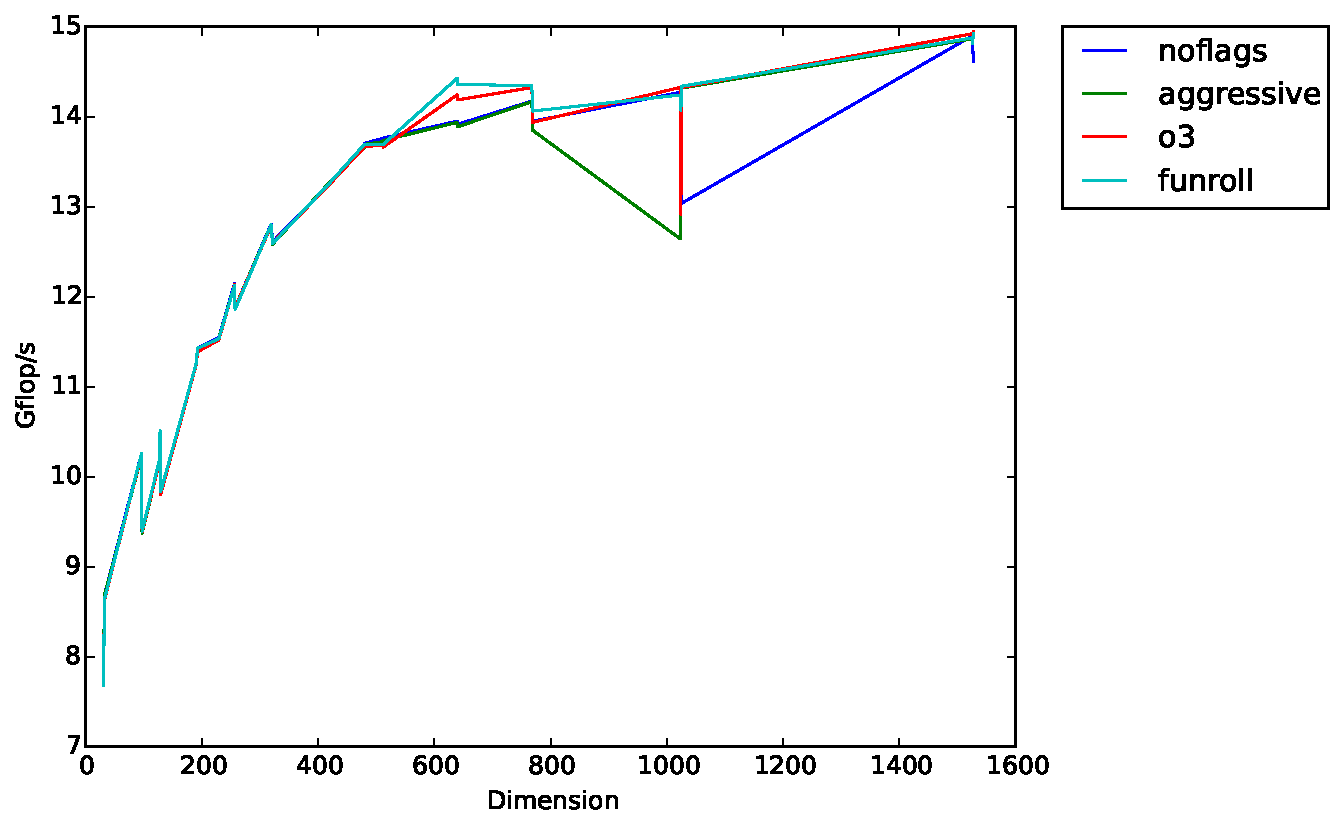
\includegraphics[width=.6\linewidth]{timing-flags_noblocking.pdf}
	\caption{Effect of compiler flags on the non-blocked AVX code.}
	\label{fig:avx-flags-noblocking}
\end{figure}

\begin{figure}[H]
	\centering
	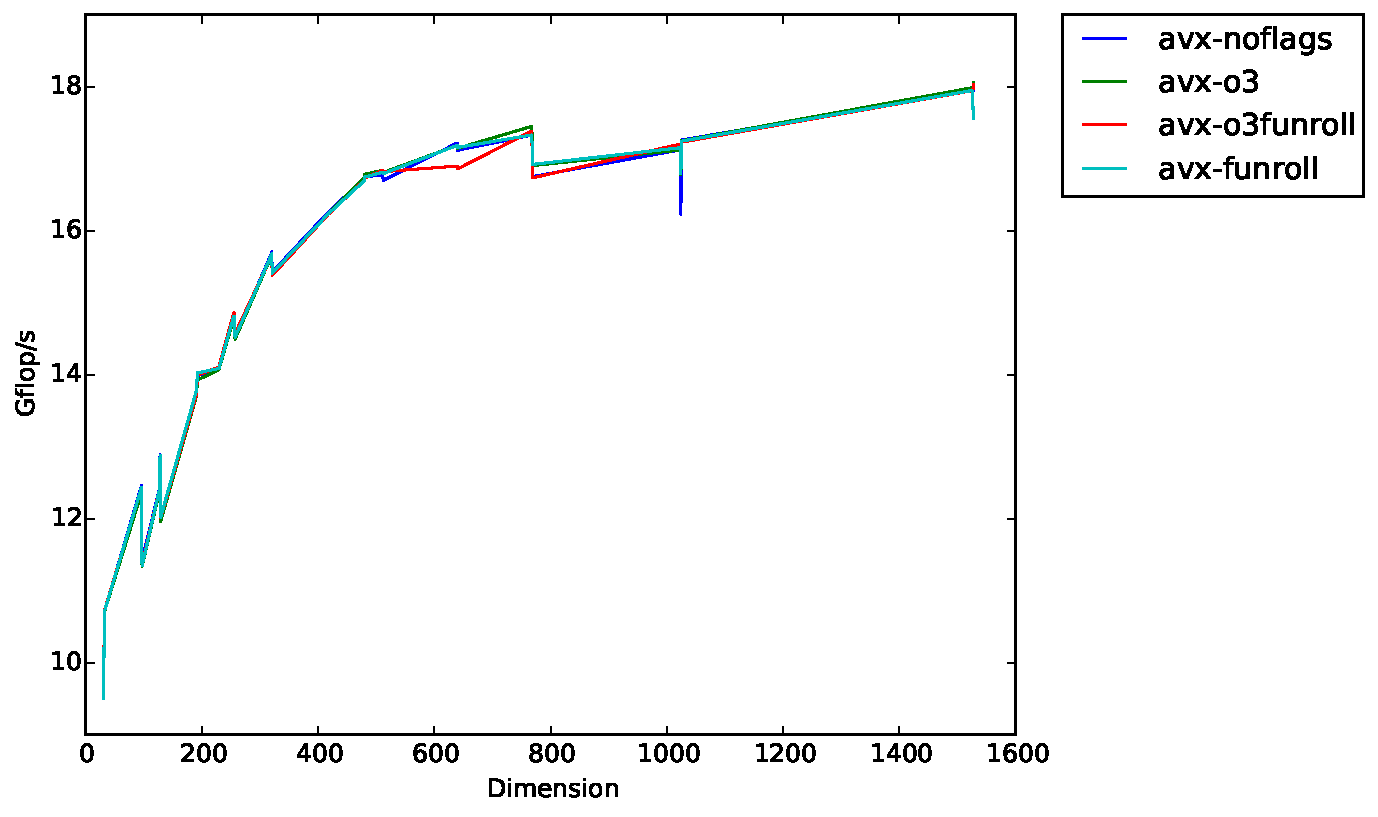
\includegraphics[width=.6\linewidth]{timing-flags_blocking.pdf}
	\caption{Effect of compiler flags on the AVX code with blocking}
	\label{fig:avx-flags-blocking}
\end{figure}

In both cases, the flags made only marginal differences. For the non-blocked version -funroll seemed to help the most, but for the blocked version -O3 was slightly better, and a combination of -O3 and -funroll was actually worse. We decided to keep only the -O3 flag for our code.

\section{Conclusion}

After adding these optimizations to our AVX-based implementation, we compared it again with the BLAS, F2C, and MKL libraries, as well as with our optimized code from Stage 1. Figure \ref{fig:final-stage2} shows this comparison, where ``mine'' is the implementation we wrote for Stage 1 and ``avx'' is our final AVX-based code. We significantly outperformed our Stage 1 code, and achieved about 50\% of the speed of MKL. We were also able to again smooth out the performance curve compared to earlier versions of our code (and even compared to MKL), making the dips at powers of 2 negligible. 

\begin{figure}[H]
	\centering
	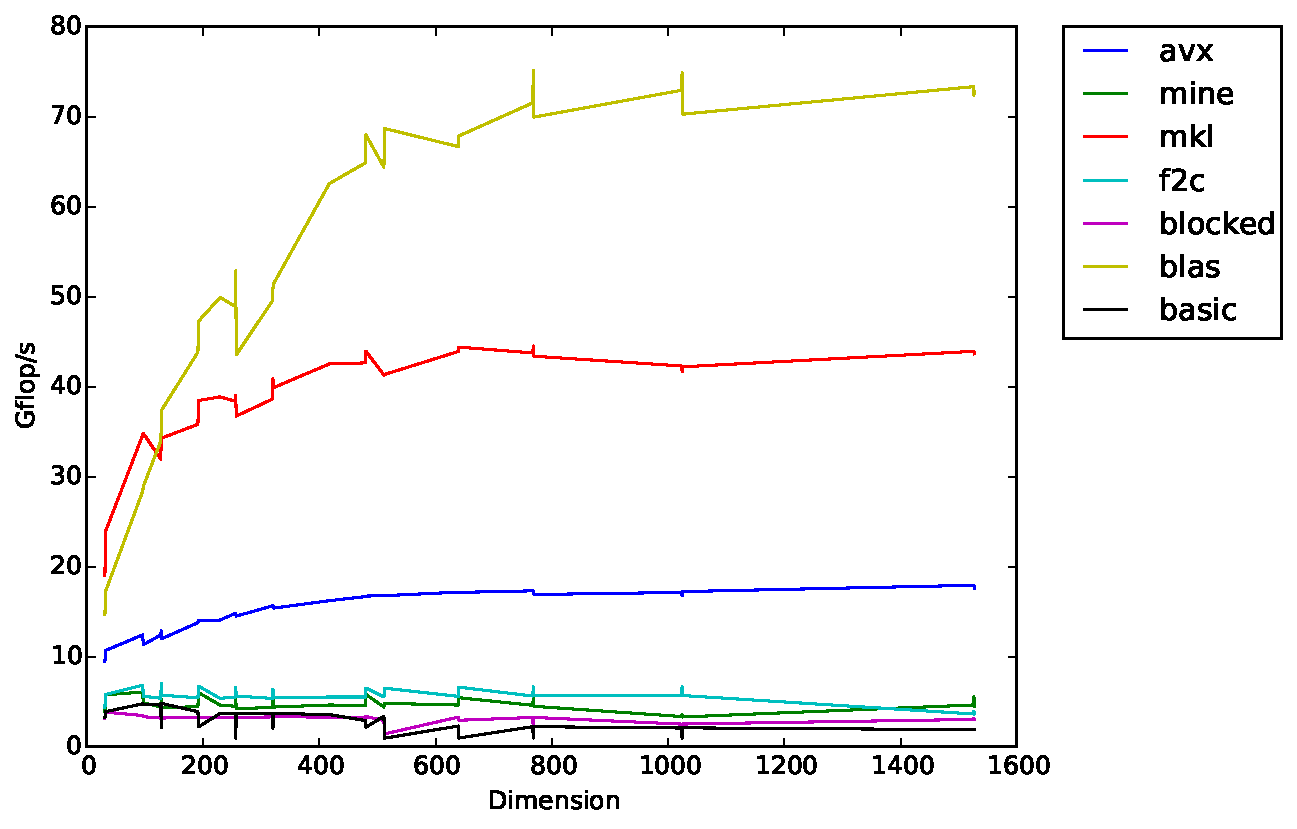
\includegraphics[width=.6\linewidth]{timing-stage2final.pdf}
	\caption{Comparison of our optimized code with other implementations, including our own previous code.}
	\label{fig:final-stage2}
\end{figure}

We realize, of course, that our implementation is still not perfect. If we had had more time to work on it, we could have experimentally tuned the size of the large blocks. We were also interested in testing the effects of transposing the matrices in the AVX code, but did not have time to implement this functionality. Future work still remains in finding the best optimizations.

\end{document}
